\section{Evaluation}
\label{sec:evaluation}

\begin{figure*}[t!]
	\centering
	\begin{minipage}{.31\textwidth}
		\centering
		\subfloat[Intra-server throughput]{                    
			%\begin{minipage}{0.4\textwidth}
			\centering
			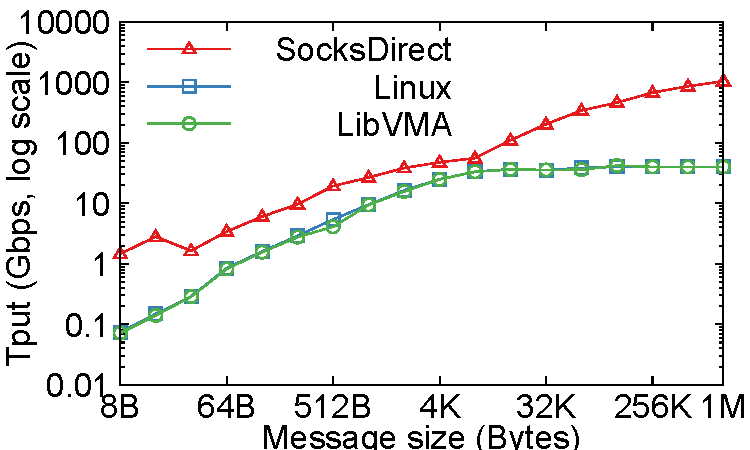
\includegraphics[width=\textwidth]{eval/microbenchmark/msgsize-ipc-tput.pdf}
			\label{fig:eval-msgsize-ipc-tput}
			%\end{minipage}
		}
		
		\subfloat[Intra-server latency]{
			%\begin{minipage}{0.4\textwidth}
			\centering 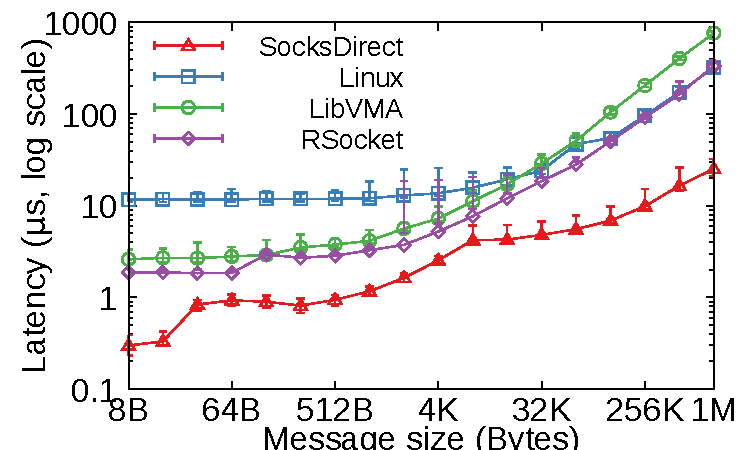
\includegraphics[width=\textwidth]{eval/microbenchmark/msgsize-ipc-lat.pdf}
			\label{fig:eval-msgsize-ipc-lat}
			%\end{minipage}
		}
		\caption{Single-core intra-server performance with message sizes.}
		\label{fig:eval-msgsize-intra}
	\end{minipage}
	\hspace{0.01\textwidth}
	\begin{minipage}{.31\textwidth}
		\centering
		\subfloat[Inter-server throughput]{
			%\begin{minipage}{0.4\textwidth}
			\centering 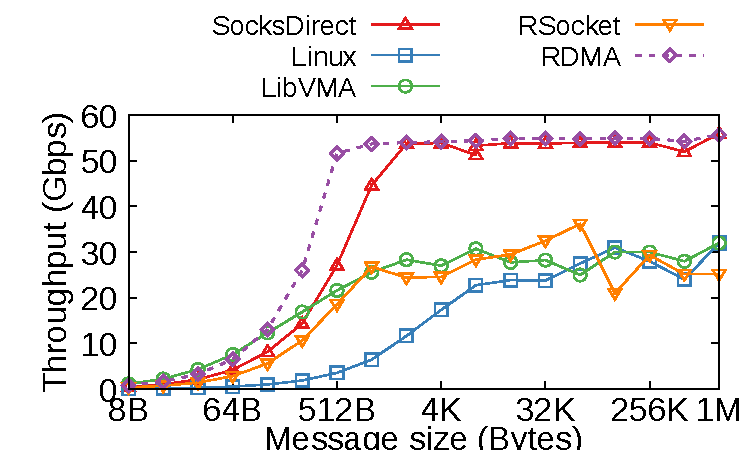
\includegraphics[width=\textwidth]{eval/microbenchmark/msgsize-network-tput.pdf}
			\label{fig:eval-msgsize-network-tput}
			%\end{minipage}
		}
		
		\subfloat[Inter-server latency]{
			%\begin{minipage}{0.4\textwidth}
			\centering 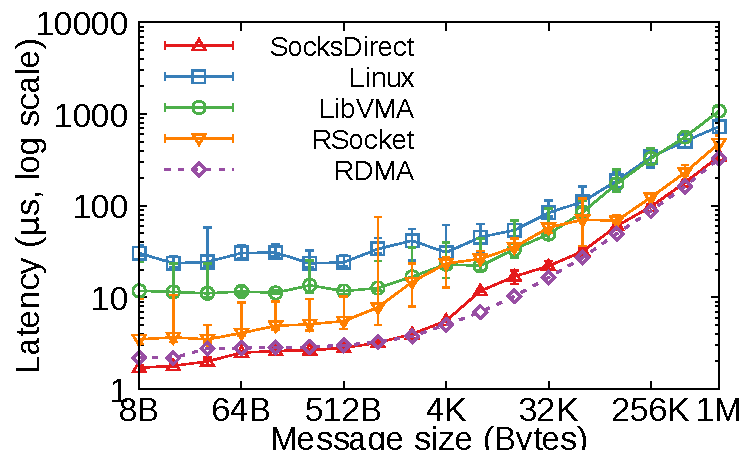
\includegraphics[width=\textwidth]{eval/microbenchmark/msgsize-network-lat.pdf}
			\label{fig:eval-msgsize-network-lat}
			%\end{minipage}
		}
		\caption{Single-core inter-server performance with message sizes.}
		\label{fig:eval-msgsize-inter}
	\end{minipage}
	\hspace{0.01\textwidth}
	\begin{minipage}{.31\textwidth}
		\centering
		\subfloat[Intra-server]{                    
			%\begin{minipage}{0.4\textwidth}
			\centering
			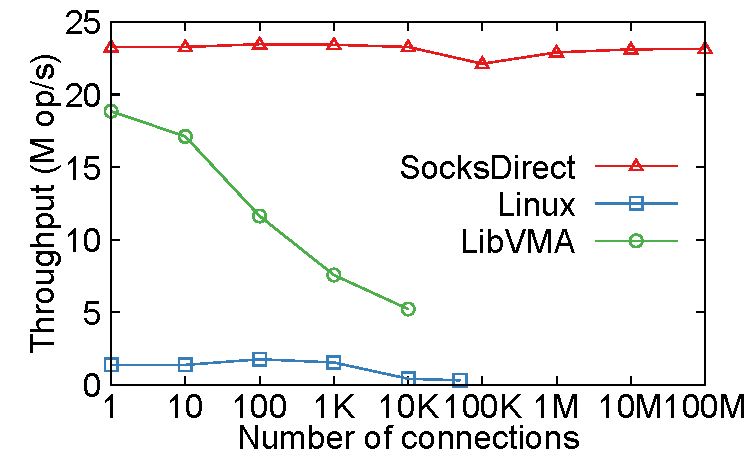
\includegraphics[width=\textwidth]{eval/microbenchmark/connnum-ipc-tput.pdf}
			\label{fig:eval-connnum-ipc-tput}
			%\end{minipage}
		}
		
		\subfloat[Inter-server]{
			%\begin{minipage}{0.4\textwidth}
			\centering 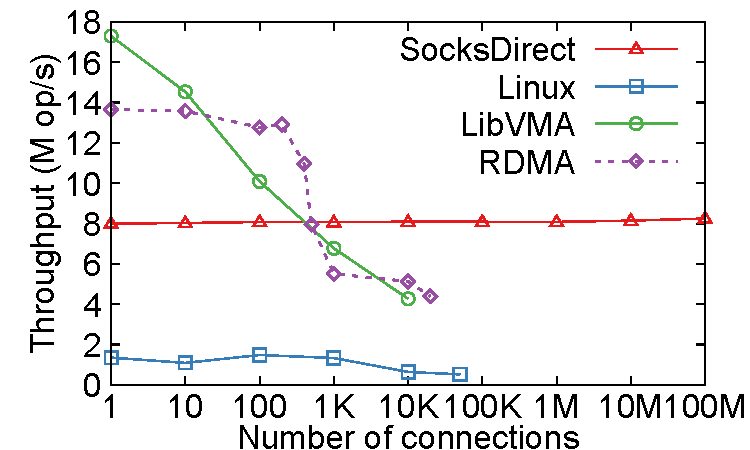
\includegraphics[width=\textwidth]{eval/microbenchmark/connnum-network-tput.pdf}
			\label{fig:eval-connnum-network-tput}
			%\end{minipage}
		}
		\caption{Single-core throughput with number of connections.}
		\label{fig:eval-connnum-tput}
	\end{minipage}
\end{figure*}

%\begin{figure}[htpb]
%	\centering
%	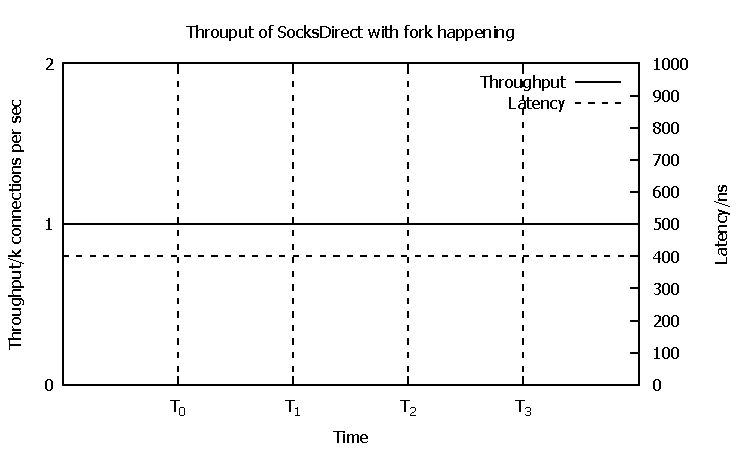
\includegraphics[width=\columnwidth]{eval/microbenchmark/fork-tput.pdf}
%	\caption{Throughput of SocksDirect with fork happening}
%	\label{fig:eval-fork-tput}
%\end{figure}


We implement \sys in three components: a userspace library \libipc{} with 10K lines of C/C++ code, a monitor program and three system calls for zero copy. 
In this section, we evaluate \sys in the following aspects:

\parab{Use shared memory efficiently for intra-server socket.}

\parab{Use RDMA efficiently for inter-server socket.}

\parab{Scale with number of connections.}

\parab{Scale with number of cores.}

\parab{Corner-case operations does not affect long-term performance.}
After slow operations.



\subsection{Methodology}

We evaluate \sys on servers with two Xeon E5-2698 v3 CPUs, 256~GiB memory and a Mellanox ConnectX-4 NIC. The servers are interconnected via an Arista 7060CX switch. We use RoCEv2 for RDMA.
Each thread is pinned on a CPU core. We run tests for enough warm-up rounds before collecting data. For latency, we report the mean, and error bars represent 1\% and 99\% percentile.

\subsection{Efficiency}



Figure~\ref{fig:eval-msgsize-intra} shows throughput and latency with different message sizes for intra-server communication. Key points: a) shared memory is faster than NIC hairpin, b) user space is faster than kernel, c) zero copy for large messages.

Figure~\ref{fig:eval-msgsize-inter} shows throughput and latency with different message sizes for inter-server communication. Key points: a) RDMA is faster than DPDK + user-space stack, b) zero copy for large messages.






\subsection{Scalability}


Figure~\ref{fig:eval-connnum-tput} shows throughput with different number of concurrent connections (log scale on x axis). Key points: a) SocksDirect is scalable with number of connections, b) other systems with one queue per socket has performance degradation under high concurrency.

Figure~\ref{fig:eval-corenum-tput} shows throughput with different number of cores for intra-server communication. Key points: a) SocksDirect is scalable with number of cores, b) NIC hairpin is not scalable with number of cores.

Figure~\ref{fig:eval-conn-setup-tput} shows throughput of connection creation. Key points: a) FastSocket not fast enough, b) higher throughput, c) scalable with number of cores.

\subsection{Deep Dive}

throughput and latency with \texttt{fork}. At time $T_0$, receiver forks, and the parent process keeps receiving. At time $T_1$, the child process begins to receives takes over the socket. At time $T_2$, sender forks, and only the parent sends. At time $T_3$, the child sender also starts sending.


Table~\ref{fig:eval-context-switch} shows throughput and latency with a dispatcher process on core $A$, multiple worker processes on core $B$ and a reducer process on core $C$. Key points: a) When all workers are active, throughput is comparable with single worker. b) When only a fraction of workers are active, the idle workers do not impact performance. c) Latency increases with number of active workers, but still much lower than Linux.